\documentclass[10pt]{article}
\usepackage[margin=0.73in]{geometry}
\usepackage{amsmath,amssymb,graphicx,booktabs,xcolor,hyperref}
\definecolor{ink}{HTML}{253C59}
\hypersetup{colorlinks=true,urlcolor=ink,linkcolor=ink}
\setlength{\parindent}{0pt}\setlength{\parskip}{6pt}
\begin{document}
{\Large\bfseries\color{ink} Direct original-point replay}\par
{\small 23 November 2026 \quad Native adapter and one capped public query}

\textbf{Implemented.} A separate Rust adapter exports the unchanged original
six-member TargetCircuit System directly: one SMT variable per original
variable, one equality per sparse polynomial row. The public query receives
only Spec, $R$, $Q=[8]R$ and limits. It checks complete model bindings and
canonical values, all original equations, then original raw-index, sign and
group replay. Arbitrary caller-built Systems are outside this public API.
[pcc:PCC-20261123-2033f1]

\begin{center}
\begin{tabular}{p{0.39\linewidth}p{0.51\linewidth}}
\toprule Fixed development control & Observed outcome\\\midrule
12 supplied complete models & Original equation/index/group replay passes; bounded corruptions refuse. Not discovery.\\
Toy and original-q/k20633 full assignments & Every value asserted to backend; SAT and replay pass. Not discovery.\\
Small native SAT/UNSAT pair & SAT model checked; UNSAT sends no get-value request.\\
Native output-cap control & Explicit truncation and refusal.\\
One public p101/q3/k8 point query & Timeout diagnostic; no status/model; no retry.\\\bottomrule
\end{tabular}
\end{center}

\textbf{Public query.} $R=(89,27)$, $Q=(70,41)=[8]R$; 327 variables,
357 quadratic equations, 1139 terms. No known unknowns enter this query.
Under the frozen 5000ms child limit, stderr is
\texttt{cvc5 interrupted by timeout.} The adapter records native signal 6 and
the separate BrokenPipe transport error. It sends no get-value request.
Outcome: resource/backend refusal. No absence, hardness, solver rate or
exponent follows. [pcc:PCC-20261123-2033f1]

\textbf{Evidence.} Final three release tests, fmt and strict all-target Clippy
pass locally. The 95-input source context is three archives: unchanged 76,
unchanged 9 and new 10 inputs. All source hashes/archive roundtrips and eight
new compiled-in hashes match. Separate write-once build/precall/postcall and
matching retained executable pre/post hashes. The 54020-byte native archive
roundtrips every captured stream; overflow capture is explicitly truncated.
The fixed shell call exits 0 while its public curve query refuses. All standing
is unsigned/not\_covered; these are local checks, not hosted gates.
[pcc:PCC-20261123-2033f1]

\textbf{Domain fidelity.} The point circuit fixes the sum of eightfold images
to $Q$. The section circuit fixes a raw pretarget sector through $R$.
Equal $Q$ alone does not establish identical search spaces. The earlier
3511-variable section cap and this 327-variable point cap therefore do not
constitute a paired performance comparison. [pcc:PCC-20261123-2033f1]

\newpage
{\large\bfseries\color{ink} Next: eliminate a specific coefficient block}
\begin{center}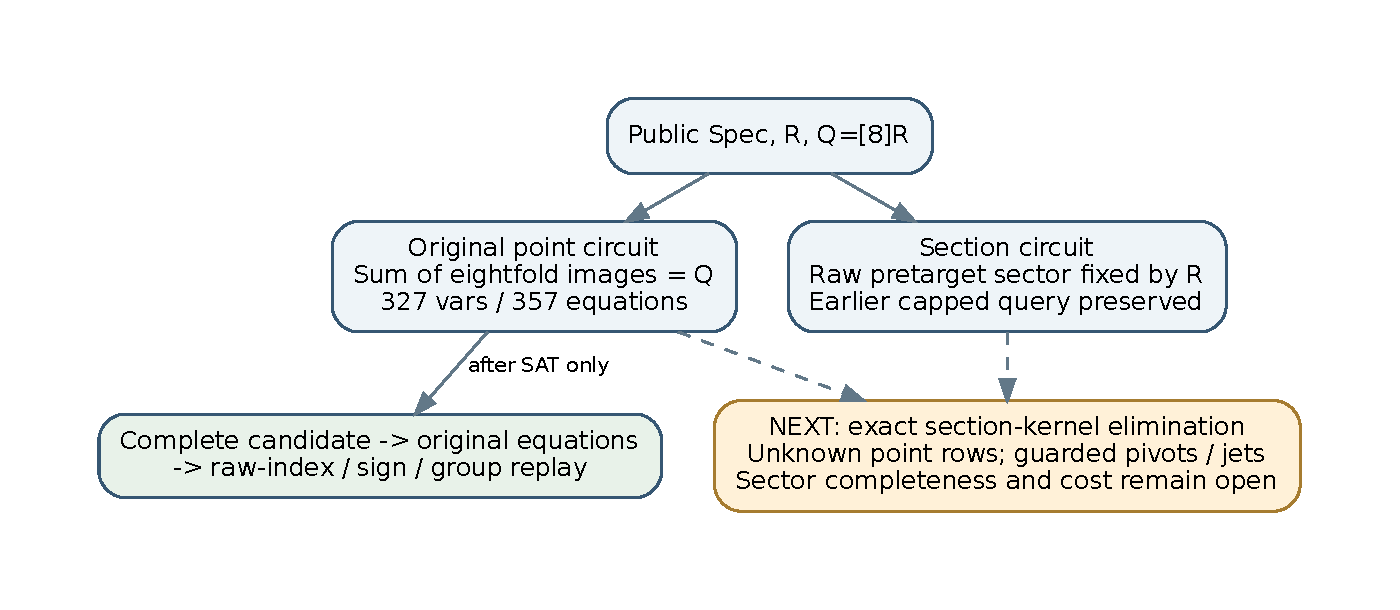
\includegraphics[width=0.93\linewidth,height=2.55in,keepaspectratio]{diagram.pdf}\end{center}

\textbf{Existing operation.} The repository already implements a six-section
evaluation kernel for supplied tuples, with repeated-point Hasse jets,
target-pole and removable-pole charts. Classical section evaluation and
linear algebra are not novel. Reconstructing coefficients after guessing all
six points does not discover an unknown tuple. [pcc:unverified]

\textbf{Proposed compiler operation.} Compile those rows for unknown original
point coordinates. Reconstruct five coefficients only on explicit nonzero
pivot-minor charts, preserving the normalized chart and every original guard.
Keep the original equations as exact fallback on unresolved/rank-deficient
strata. Preserve aliases, multiplicities and both target charts. First match
or charge raw-$R$ sector completeness. See NEXT.md for acceptance conditions.
This operation is not implemented or proved here. [pcc:unverified]

\textbf{Discriminating obligations.} Establish extension/projection against
the original circuit and numeric section predicate, then count branch work,
fill, degrees, live memory and original lifting/setup. Fewer coefficient
variables or a fixed-size kernel alone supplies no solving-degree or search
bound. Useful target yield, relation rank, private selection, kernel/recovery,
indexing and the full growing-family cold-cost contract remain open.
No campaign or paid worker is scheduled. [pcc:unverified]

\textbf{Sources.} Native statement PCC-20261123-2033f1.\par
Evidence: PROTOCOL.md and FIDELITY.md.\par
Source identity: SOURCE\_QUALIFICATION.json; native raw manifest.\par
Cheng, \emph{Hard Problems of Algebraic Geometry Codes},
\href{https://arxiv.org/pdf/cs/0507026}{cs/0507026}, \S2/Theorem1;
Snowden, \href{https://websites.umich.edu/asnowden/teaching/2013/679/L02.html}{Math679 lecture2}.
Backend context: Ozdemir et al., CAV2024,
\href{https://theory.stanford.edu/~barrett/pubs/OPB+24.pdf}{Split Gr\"obner Bases};
\href{https://cvc5.github.io/docs/cvc5-1.4.2/theories/finite_field.html}{pinned cvc5 theory reference}.
KB unavailable; bounded review establishes no novelty. No new Lean endpoint
or formal compiler/group/cost theorem. Old artifact access, immutable-record
and journal integration obligations remain open; original evidence and
criteria are unchanged.
\end{document}
